%Plantilla para proyectos modulares de ciencias básicas.
%Para usar en los proyectos de Lic. en Física. Para otras carreras consulte a su coordinador.
%
%Edite donde se indica y sea necesario.
%
%Versión 2.0
%


\documentclass[letterpaper,12pt]{article}
\usepackage[utf8]{inputenc}
\usepackage[table]{xcolor}
\usepackage{graphicx}
\usepackage{epsfig}
\usepackage{float}
\usepackage[hidelinks]{hyperref}
\usepackage{array}
\usepackage{lastpage}
\usepackage[spanish,es-tabla]{babel} % Se considera TABLA en lugar de CUADRO en las tablas. Modificado por Rotosca
\usepackage{fancyhdr}
\usepackage{geometry}

%Matemática
\usepackage{amsmath}
\usepackage{amsfonts}
\usepackage{amssymb}
\usepackage{tabularx}
\usepackage{multicol}
\usepackage{soul}
\usepackage{amstext}


%tamaño de la fuente en las secciones.
\usepackage{sectsty}
\sectionfont{\fontsize{12}{15}\selectfont}
\subsectionfont{\fontsize{11}{15}\selectfont}


\definecolor{AzulModular}{cmyk}{1.0,0.49,0.0,0.47}%color #4365A4

\setlength{\parindent}{0.95cm}

\geometry{
  left=0.748in,
  right=0.780in,
  top=3.9cm,
  headheight=1.9cm,
  headsep=0.5cm,
%  bottom=3.54cm,
  footskip=2.54cm,
}

\decimalpoint

\graphicspath{{../figuras/}}

\newcommand{\cfbox}[2]{%
    \colorlet{currentcolor}{.}%
    {\color{#1}%
    \fbox{\color{currentcolor}#2}}%
}


\pagestyle{fancy}
\cfoot{}
\renewcommand{\headrulewidth}{0pt}
\fancyhead[CO,LO,RO]{} %% clear out all headers
\fancyhead[C]{%
          \begin{tabular}{m{1.5cm}m{11.5cm}m{2.5cm}}
          
\includegraphics[height=1.5cm]{udg_4365A4} &\cellcolor{AzulModular}
          \centering
          \cfbox{white}{%
            \begin{minipage}{10.5cm}
              \centering
              \textcolor{white}{Evaluación Modular, Departamento de Física, 2026B}
            \end{minipage}
            }
            &
          \centering
          \tiny{Licenciatura en Física\\%para usar en otras carreras consulte a su coordinador
%%%%%%%%%%%%%%%%%%%%%%%%%%%%%%%%%%%%%%%%%%%%%%%%%%%%%%%%%%%%%%%%%%%%%%%%%%%%%%%%%%%%%%%%%%%%%%%%%
            Modular: [I, II o III]\\ %elija el que corresponda ejemplo :  Modular : I
%%%%%%%%%%%%%%%%%%%%%%%%%%%%%%%%%%%%%%%%%%%%%%%%%%%%%%%%%%%%%%%%%%%%%%%%%%%%%%%%%%%%%%%%%%%%%%%%%
            Página \thepage \hspace{1pt} de \pageref{LastPage}\\
          }\tabularnewline
%          \hline
          \end{tabular}%
}

%%%%%%%%%%%%%%%%%%%%%%%%%%%%%%%%%%%%%%%%%%%%%%%%%%%%%%%%%%%%%%%%%%%%%%%%%%%%%%%%%%%%%%%%%%%%%%%%%
\title{\fontsize{0.5cm}{0.5cm}\selectfont
\textit{\textbf{La desigualdad aparece sola: mecánica estadística del dinero en un modelo de intercambio aleatorio}}
}
\author{ \fontsize{0.35cm}{0.5cm}\selectfont
\textit{Luis Alberto Román Verde$^1$} \\
        \and \fontsize{0.35cm}{0.5cm}\selectfont \textit{\textbf{Asesor:} [Nombre del asesor]$^1$}
	}

\date{\small
  $^1$\fontsize{0.35cm}{0.5cm}\selectfont \textit{luis.roman4456@alumnos.udg.mx\\ Departamento de Física, CUCEI, Universidad de Guadalajara\\
    Blvd. Marcelino García Barragán 1421, Col. Olímpica, Guadalajara Jal., C. P. 44430, México}\\[2ex]
  }
%%%%%%%%%%%%%%%%%%%%%%%%%%%%%%%%%%%%%%%%%%%%%%%%%%%%%%%%%%%%%%%%%%%%%%%%%%%%%%%%%%%%%%%%%%%%%%%%%

%%%%%%%%%%%%%%%%%%%%%%%%%%%%%%% Comienza el documento%%%%%%%%%%%%%%%%%%%%%%%%%%%%%%%%%%5
\begin{document}
\maketitle
\thispagestyle{fancy}

\section*{Resumen}
Se estudia, como trabajo introductorio, el modelo de intercambio aleatorio de Drăgulescu y Yakovenko, que trata a las personas de una economía como las moléculas de un gas y al dinero como su energía. En el modelo, $N$ personas empiezan con exactamente la misma cantidad de dinero y realizan intercambios al azar en los que el dinero total se conserva y nadie puede endeudarse. Se muestra, primero contando de manera exacta todos los repartos posibles y después con una simulación numérica de 2000 personas y $4\times10^{6}$ intercambios, que el sistema pasa espontáneamente de la igualdad perfecta a una distribución exponencial de Boltzmann, $P(m)\propto e^{-m/T}$, donde la ``temperatura'' $T$ es el dinero promedio por persona. La entropía crece hasta su valor máximo y el coeficiente de Gini sube de 0 a $0.508\pm0.004$, en acuerdo con el valor teórico $\approx0.51$ (exactamente $1/2$ para dinero continuo). El resultado no depende del número de personas, del dinero inicial ni de la regla concreta de intercambio. Se explica por qué los estados de poco dinero son los más probables: cada moneda que acumula una persona reduce exponencialmente las formas en que el resto puede repartirse el dinero. Todos los datos de este trabajo son simulados. Se plantea, como hipótesis para trabajo posterior, que la desigualdad observada en el mundo real excede la que produciría el azar.

\section*{Introducción}
La desigualdad económica es uno de los temas centrales de la economía política y de las relaciones internacionales: se discute entre países y dentro de ellos, y se asocia con conflictos, migración y estabilidad política. Suele explicarse con causas particulares, como diferencias de educación, de capital heredado, de instituciones o de poder. Este trabajo plantea una pregunta previa y más básica: \emph{si todas las personas fueran idénticas y siguieran exactamente las mismas reglas, ¿se mantendría la igualdad?}

La física estadística ofrece una respuesta sorprendente. En un gas, todas las moléculas son idénticas y obedecen las mismas leyes; sin embargo, en equilibrio, sus energías no son iguales: la mayoría tiene poca energía y unas pocas tienen mucha. Esa distribución, la ley de Boltzmann, no es consecuencia de ninguna diferencia entre moléculas, sino de cuántas maneras hay de repartir la energía total \cite{reif}. En el año 2000, Drăgulescu y Yakovenko propusieron aplicar exactamente esta idea al dinero \cite{dy2000}: las personas son las moléculas, el dinero es la energía y cada compra o venta es un choque en el que el dinero pasa de una persona a otra sin crearse ni destruirse.

El objetivo de este trabajo introductorio es (i) explicar con claridad por qué, en este modelo, la desigualdad aparece sola, (ii) aclarar qué significa físicamente que los ``estados de menor energía'' sean los más probables y cómo se traduce eso al dinero, y (iii) verificarlo con una simulación propia. \textbf{Todos los datos que se presentan son simulados}; no se utilizan todavía datos económicos reales. Su comparación con datos reales se deja para una etapa posterior.

\section*{Marco teórico}

\subsection*{La analogía entre moléculas y personas}
La Tabla~\ref{tab:analogia} resume la correspondencia en la que se basa el modelo \cite{dy2000,yr2009}. La pieza clave es la conservación: en un intercambio comercial, el dinero que pierde el comprador es exactamente el que gana el vendedor, igual que la energía en un choque elástico. Solo las autoridades monetarias crean o destruyen dinero, lo cual se ignora en este modelo, del mismo modo que se ignora el intercambio de energía con el exterior en un gas aislado.

\begin{table}[H]
  \begin{center}
    \begin{tabular}{|l|l|}
      \hline
      \textbf{Gas ideal} & \textbf{Economía del modelo} \\
      \hline \hline
      Molécula & Persona \\
      \hline
      Energía de una molécula, $\varepsilon$ & Dinero de una persona, $m$ \\
      \hline
      Choque entre dos moléculas & Compra-venta entre dos personas \\
      \hline
      Energía total constante & Dinero total $M$ constante \\
      \hline
      Energía nunca negativa & Sin deudas: $m\geq0$ \\
      \hline
      Temperatura $k_BT$ & Dinero promedio $T=M/N$ \\
      \hline
      Equilibrio térmico & Distribución estacionaria del dinero \\
      \hline
      Entropía & Número de formas de repartir el dinero \\
      \hline
    \end{tabular}
  \end{center}
  \caption{Correspondencia entre un gas y el modelo de intercambio de dinero.}
  \label{tab:analogia}
\end{table}

La analogía también tiene límites, que se discuten al final: las personas no son idénticas, no intercambian al azar, producen, ahorran, heredan y cobran intereses. El modelo no pretende describir todo eso; pretende aislar el efecto del puro azar.

\subsection*{Contar repartos: el origen de la desigualdad}
Supóngase que hay $N$ personas y $M$ monedas idénticas, y que el sistema ha intercambiado tanto que cualquier reparto es igual de probable (\emph{postulado de igual probabilidad a priori} \cite{reif}). El número de formas de repartir $M$ monedas entre $N$ personas es
\begin{equation}
  \Omega(N,M)=\binom{M+N-1}{N-1}.
  \label{eq:omega}
\end{equation}
Si una persona en particular tiene $m$ monedas, las $M-m$ restantes se reparten entre las otras $N-1$ personas de $\Omega(N-1,M-m)$ maneras. Por lo tanto, la probabilidad de que esa persona tenga $m$ monedas es
\begin{equation}
  P(m)=\frac{\Omega(N-1,\,M-m)}{\Omega(N,M)}.
  \label{eq:pexacta}
\end{equation}
El caso más pequeño lo hace evidente. Con 3 personas y 3 monedas hay $\Omega(3,3)=10$ repartos. Una persona tiene 0 monedas en 4 de ellos, 1 moneda en 3, 2 monedas en 2 y las 3 monedas en solo 1. Las probabilidades son 40\%, 30\%, 20\% y 10\%: \textbf{lo más probable es tener poco}, aunque nadie tenga ventaja alguna sobre los demás.

\subsection*{¿Qué significa que los estados de menor energía sean los más probables?}
En física se suele decir que, a temperatura $T$, un estado de energía $\varepsilon$ tiene probabilidad proporcional a $e^{-\varepsilon/k_BT}$, de modo que los estados de menor energía son los más probables. Es importante entender \emph{por qué}, porque de ahí sale la interpretación económica.

La molécula no ``prefiere'' tener poca energía. Lo que ocurre es que la molécula forma parte de un sistema mucho más grande, el resto del gas, que actúa como \emph{reservorio}. Toda la energía que tiene la molécula es energía que le falta al reservorio, y el reservorio con menos energía tiene muchas menos formas de organizarse. Escribiendo el logaritmo del número de formas del resto y desarrollando para $m\ll M$,
\begin{equation}
  \ln\Omega(N-1,\,M-m)\approx\ln\Omega(N-1,\,M)-m\,\frac{\partial\ln\Omega}{\partial M}
  \equiv\ln\Omega(N-1,\,M)-\frac{m}{T},
  \label{eq:reservorio}
\end{equation}
de donde
\begin{equation}
  P(m)\propto e^{-m/T},\qquad \frac{1}{T}=\frac{\partial\ln\Omega}{\partial M}.
  \label{eq:boltzmann}
\end{equation}
Esta es precisamente la definición estadística de temperatura: qué tan rápido crece el número de configuraciones al agregar energía. Para el modelo de dinero, usando la ec.~\ref{eq:omega} con $N,M\gg1$, se obtiene $1/T\approx\ln(1+N/M)$, que para $M\gg N$ da $T\approx M/N$: la temperatura del dinero es el dinero promedio por persona \cite{dy2000}.

Traducido al lenguaje social: \textbf{cada moneda que una persona acumula es una moneda que el resto de la sociedad ya no puede repartirse}, y eso reduce de forma exponencial el número de situaciones compatibles. Por eso, en un instante dado, la mayoría de las personas tiene poco dinero y muy pocas tienen mucho. No se trata de un juicio sobre mérito ni de un destino individual: es un enunciado sobre \emph{qué fracción} de la población se encuentra, en cada momento, en cada nivel de dinero.

\subsection*{Máxima entropía}
El mismo resultado se obtiene pidiendo que la entropía $S=-\sum_m P(m)\ln P(m)$ sea máxima con dos restricciones: que las probabilidades sumen uno y que el dinero promedio sea $T$. Con multiplicadores de Lagrange $\alpha$ y $\beta$,
\begin{equation}
  \frac{\partial}{\partial P(m)}\left[S-\alpha\Big(\sum_m P(m)-1\Big)-\beta\Big(\sum_m mP(m)-T\Big)\right]=0
  \;\Rightarrow\; P(m)=\frac{1}{T}\,e^{-m/T}.
  \label{eq:maxent}
\end{equation}
La distribución exponencial es, entonces, el reparto ``más desordenado'' posible compatible con que el dinero se conserve. Su entropía máxima es $S_{\max}=1+\ln T$ (con $m$ medido en monedas). La segunda ley de la termodinámica, aplicada aquí, dice que el sistema evolucionará desde cualquier estado inicial, incluido el de igualdad perfecta, hacia este estado de máxima entropía.

\subsection*{Cómo se mide la desigualdad}
La \emph{curva de Lorenz} $L(p)$ indica qué fracción del dinero total tiene la fracción $p$ más pobre de la población \cite{lorenz}; con igualdad perfecta $L(p)=p$. El \emph{coeficiente de Gini} $G$ es el doble del área entre la recta de igualdad y la curva de Lorenz \cite{gini}: $G=0$ si todos tienen lo mismo y $G=1$ si una sola persona lo tiene todo. Para la distribución exponencial se obtiene de forma exacta
\begin{equation}
  L(p)=p+(1-p)\ln(1-p),\qquad G=\frac{1}{2}.
  \label{eq:lorenz}
\end{equation}
Con dinero en monedas enteras de valor $\Delta m$, la distribución es geométrica y $G=1/(1+e^{-\Delta m/T})$, que tiende a $1/2$ cuando $T\gg\Delta m$. De la ec.~\ref{eq:lorenz} se derivan predicciones concretas: la mitad más pobre posee el 15.3\% del dinero, el 10\% más rico posee el 33.0\%, y una fracción $1-e^{-1}\approx63.2\%$ de las personas tiene menos que el promedio.

\section*{Metodología}

\subsection*{Naturaleza de los datos}
\textbf{Todos los datos de este trabajo son simulados por computadora.} No provienen de encuestas, registros fiscales ni cuentas bancarias. Su propósito es mostrar lo que el modelo predice en condiciones controladas, para tener una referencia contra la cual comparar datos reales en una etapa posterior.

\subsection*{Algoritmo de simulación}
Se reprodujo el modelo de la ref.~\cite{dy2000} en Python con NumPy \cite{numpy}:
\begin{enumerate}
  \item Se crean $N=2000$ personas, cada una con $m_0=20$ monedas. El estado inicial es de igualdad perfecta ($G=0$).
  \item En cada paso se eligen al azar un pagador $i$ y un receptor $j$ ($i\neq j$).
  \item Si $m_i\geq\Delta m$, el pagador entrega $\Delta m=1$ moneda al receptor; si no, el intercambio no ocurre (no hay deudas).
  \item Se repiten $4\times10^{6}$ pasos, es decir, unos 2000 intercambios por persona.
  \item Cada $10^{4}$ pasos se mide la entropía, el coeficiente de Gini y el dinero de cada persona.
  \item Al final se verifica que el dinero total siga siendo exactamente $N m_0=40\,000$.
\end{enumerate}
La entropía se calcula con las frecuencias del histograma de dinero y el Gini con la fórmula estándar sobre los valores ordenados. La semilla del generador de números aleatorios es fija, de modo que el resultado es reproducible.

\subsection*{Conteo exacto}
De manera independiente de la simulación, se evaluó la ec.~\ref{eq:pexacta} para $(N,M)=(3,3)$, $(10,50)$ y $(100,1000)$, a fin de mostrar que la forma exponencial surge de contar repartos y no de algún detalle del algoritmo.

\subsection*{Pruebas de robustez}
Para comprobar que el resultado no depende de las elecciones particulares, se repitió la simulación con 5 semillas distintas en cinco configuraciones: el caso base; menos personas ($N=500$); menos dinero inicial ($m_0=10$); más dinero y pagos más grandes ($m_0=40$, $\Delta m=2$); y una regla de intercambio distinta, en la que cada pareja junta su dinero y lo reparte con una fracción aleatoria uniforme, lo que también conserva el dinero.

\section*{Resultados}

\subsection*{El conteo exacto ya produce la desigualdad}
La Fig.~\ref{fig:conteo} muestra la probabilidad exacta de la ec.~\ref{eq:pexacta}. Con 3 personas se recupera el 40\%, 30\%, 20\%, 10\% calculado arriba. Al crecer el número de personas, el conteo se acerca a la exponencial $e^{-m/T}/T$. No interviene ninguna simulación: la desigualdad surge únicamente de contar.

\begin{figure}[H]
   \centering
   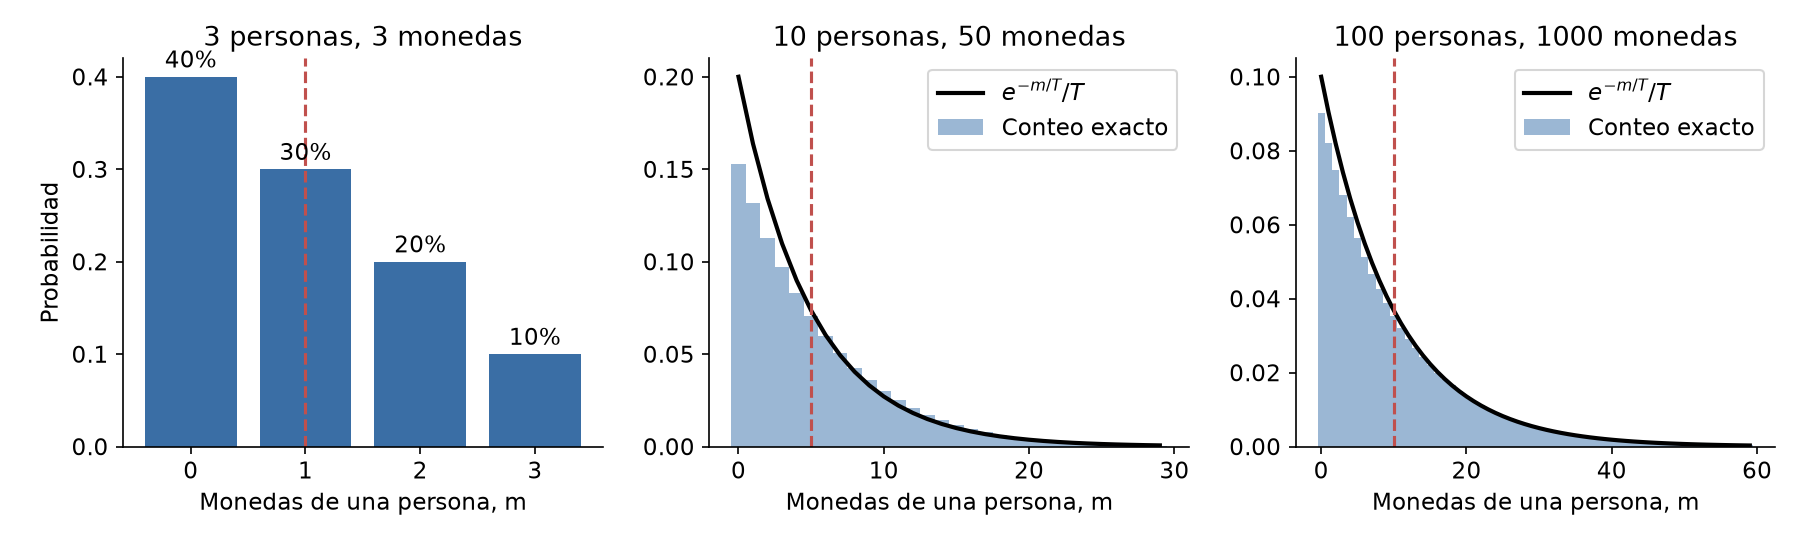
\includegraphics[width=\textwidth]{fig1_conteo_exacto}
   \caption{Probabilidad exacta de que una persona tenga $m$ monedas, obtenida contando todos los repartos posibles (ec.~\ref{eq:pexacta}). La línea roja marca el promedio. Al aumentar el tamaño del sistema el resultado se aproxima a la ley de Boltzmann.}
   \label{fig:conteo}
\end{figure}

\subsection*{Distribución final del dinero}
Aunque todas las personas empezaron con 20 monedas, al final de la simulación el dinero está repartido según la ley de Boltzmann (Fig.~\ref{fig:dist}). En escala logarítmica la exponencial es una recta, y los datos simulados la siguen; la dispersión a la derecha corresponde a niveles de dinero que tienen solo una o dos personas, es decir, a ruido estadístico. El dinero total se conservó exactamente (40\,000 monedas).

\begin{figure}[H]
   \centering
   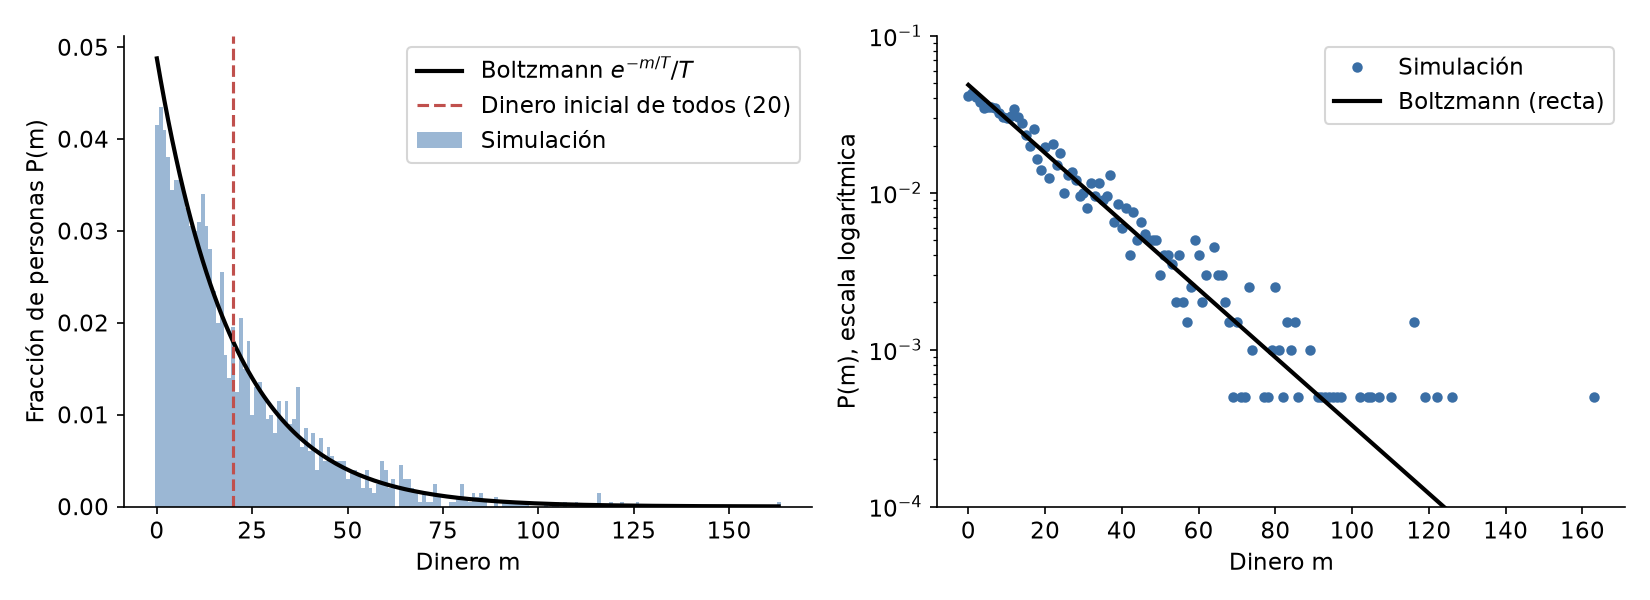
\includegraphics[width=\textwidth]{fig2_distribucion}
   \caption{Distribución del dinero tras $4\times10^{6}$ intercambios (datos simulados, $N=2000$, $m_0=20$, $\Delta m=1$). Izquierda: escala lineal; la línea roja marca el dinero inicial, igual para todos. Derecha: escala logarítmica, donde la ley de Boltzmann es una recta.}
   \label{fig:dist}
\end{figure}

\subsection*{La entropía crece y la desigualdad aparece}
La Fig.~\ref{fig:evol} muestra cómo evoluciona el sistema. La entropía parte de cero (todos tienen lo mismo, hay un solo reparto) y crece hasta su máximo teórico $S_{\max}=1+\ln 20=3.996$; al final de la simulación vale 3.978. El coeficiente de Gini sigue el mismo camino: pasa de 0 a un valor que fluctúa alrededor de 0.5 después de unos 500 intercambios por persona. Nadie hizo trampa y nadie tuvo ventaja: la desigualdad es el estado de equilibrio.

\begin{figure}[H]
   \centering
   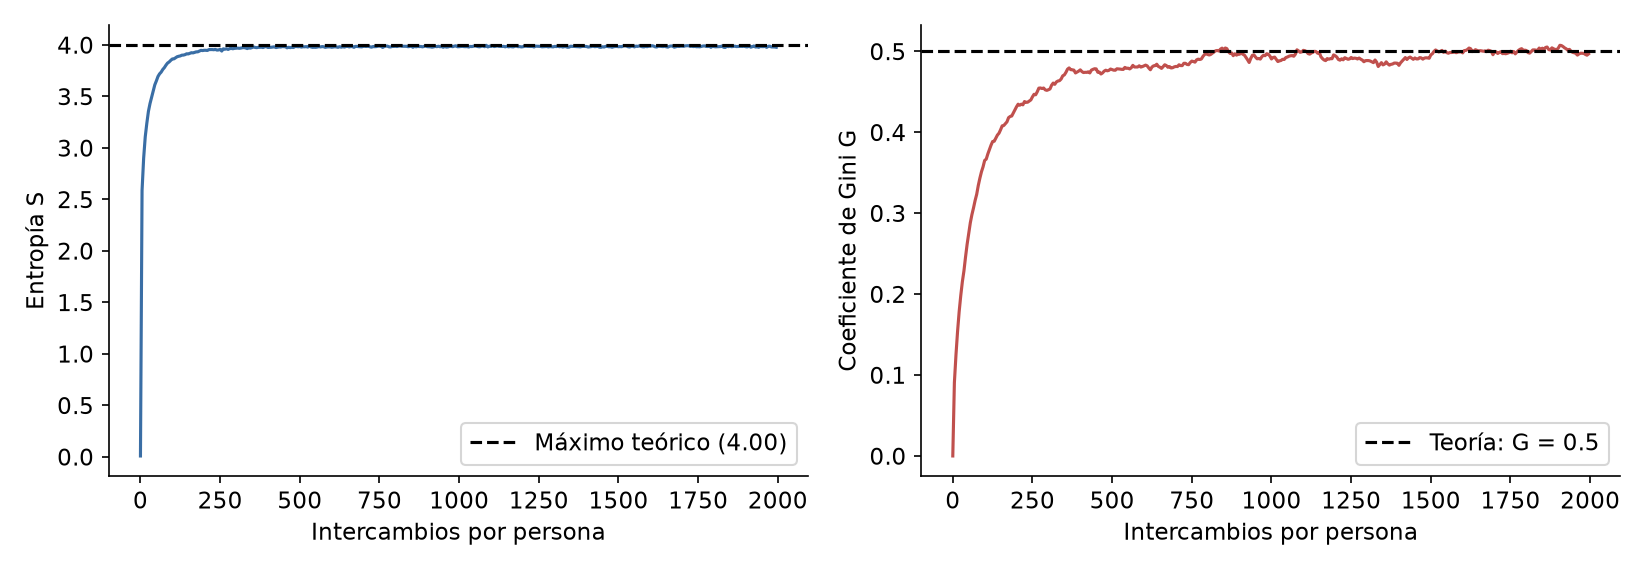
\includegraphics[width=\textwidth]{fig3_evolucion}
   \caption{Evolución de la entropía (izquierda) y del coeficiente de Gini (derecha) a lo largo de la simulación. Ambos parten del estado de igualdad perfecta y se estabilizan en los valores predichos por la ley de Boltzmann.}
   \label{fig:evol}
\end{figure}

\subsection*{Curva de Lorenz}
La curva de Lorenz final coincide con la expresión exacta de la ec.~\ref{eq:lorenz} (Fig.~\ref{fig:lorenz}). La Tabla~\ref{tab:base} compara las cantidades medidas con las predicciones teóricas.

\begin{figure}[H]
   \centering
   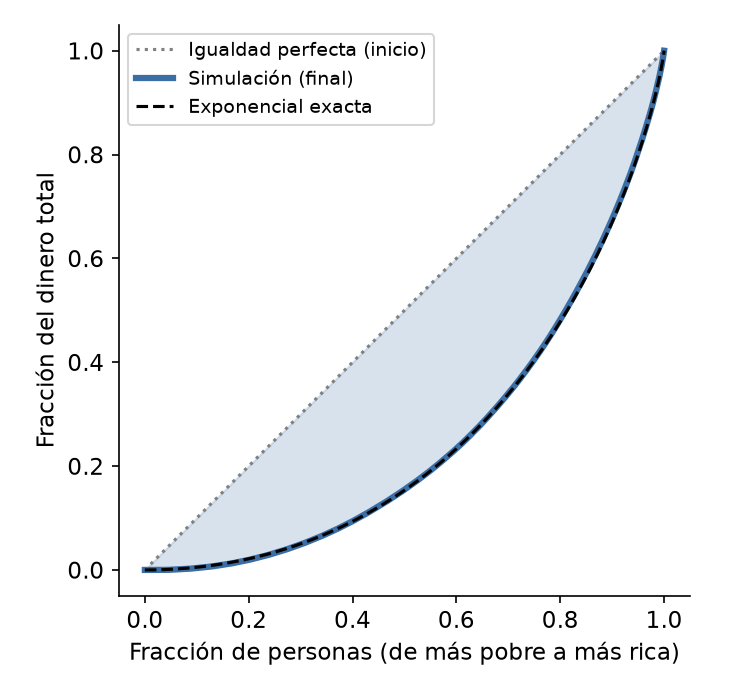
\includegraphics[width=0.5\textwidth]{fig4_lorenz}
   \caption{Curva de Lorenz al final de la simulación, comparada con la de la distribución exponencial y con la recta de igualdad perfecta (estado inicial). El área sombreada es la mitad del coeficiente de Gini.}
   \label{fig:lorenz}
\end{figure}

\begin{table}[H]
  \begin{center}
    \begin{tabular}{|l|c|c|}
      \hline
      \textbf{Cantidad} & \textbf{Simulación} & \textbf{Teoría} \\
      \hline \hline
      Dinero total & 40\,000 & 40\,000 \\
      \hline
      Coeficiente de Gini & 0.498 & 0.512 \\
      \hline
      Entropía final & 3.978 & 3.996 \\
      \hline
      Personas con menos que el promedio & 62.0\% & 63.2\% \\
      \hline
      Personas sin dinero ($m=0$) & 4.2\% & 4.9\% \\
      \hline
      Dinero de la mitad más pobre & 15.5\% & 15.3\% \\
      \hline
      Dinero del 10\% más rico & 32.4\% & 33.0\% \\
      \hline
    \end{tabular}
  \end{center}
  \caption{Caso base (datos simulados, una semilla) comparado con las predicciones de la distribución de Boltzmann. El Gini teórico corresponde a monedas discretas, $1/(1+e^{-\Delta m/T})$.}
  \label{tab:base}
\end{table}

\subsection*{Movilidad: nadie es rico o pobre para siempre}
Un aspecto que la distribución por sí sola no muestra es qué le ocurre a cada persona. La Fig.~\ref{fig:movil} sigue el dinero de tres personas: todas pasan por momentos de pobreza ($m=0$) y de riqueza (más del doble del promedio). La distribución exponencial es un equilibrio \emph{estadístico}: la forma del reparto se mantiene, pero las personas cambian constantemente de lugar dentro de él. En promedio, cada persona pasó el 61\% del tiempo por debajo del promedio, cerca del 63\% predicho; la dispersión entre personas es grande porque la ventana de observación abarca solo unos pocos tiempos de relajación.

\begin{figure}[H]
   \centering
   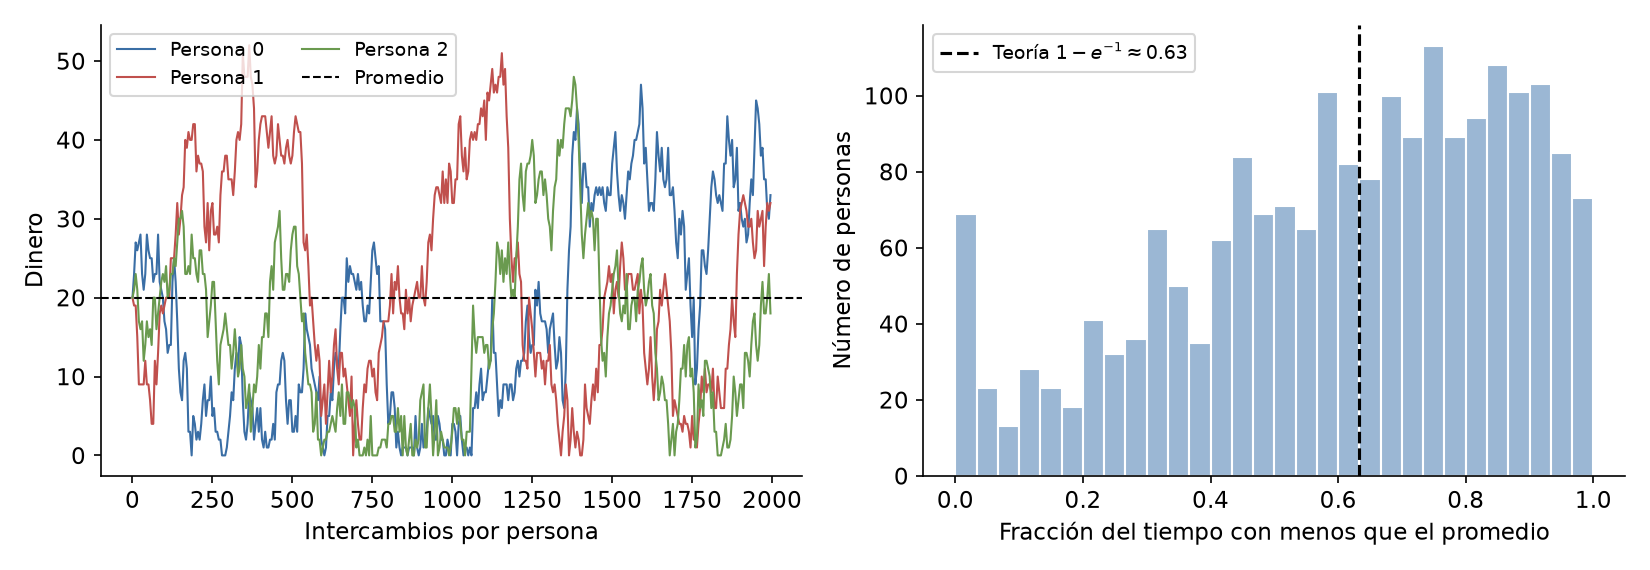
\includegraphics[width=\textwidth]{fig5_movilidad}
   \caption{Izquierda: dinero de tres personas a lo largo del tiempo. Derecha: fracción del tiempo (después de 500 intercambios por persona) que cada una de las 2000 personas pasó con menos dinero que el promedio.}
   \label{fig:movil}
\end{figure}

\subsection*{Robustez}
La Tabla~\ref{tab:robustez} muestra que el coeficiente de Gini de equilibrio no depende del número de personas, del dinero inicial, del tamaño de los pagos ni de la regla de intercambio. Las pequeñas diferencias respecto de $1/2$ se explican por el carácter discreto de las monedas y coinciden con la fórmula $1/(1+e^{-\Delta m/T})$ dentro de una o dos desviaciones estándar.

\begin{table}[H]
  \begin{center}
    \begin{tabular}{|l|c|c|c|c|c|}
      \hline
      \textbf{Configuración} & $N$ & $m_0$ & $\Delta m$ & \textbf{Gini simulado} & \textbf{Gini teórico} \\
      \hline \hline
      Base & 2000 & 20 & 1 & $0.508\pm0.004$ & 0.512 \\
      \hline
      Menos personas & 500 & 20 & 1 & $0.511\pm0.009$ & 0.512 \\
      \hline
      Menos dinero & 2000 & 10 & 1 & $0.520\pm0.008$ & 0.525 \\
      \hline
      Más dinero y pagos & 2000 & 40 & 2 & $0.508\pm0.004$ & 0.512 \\
      \hline
      Reparto aleatorio & 2000 & 20 & -- & $0.502\pm0.008$ & 0.500 \\
      \hline
    \end{tabular}
  \end{center}
  \caption{Coeficiente de Gini de equilibrio (media y desviación estándar de 5 semillas) para distintas configuraciones. Datos simulados.}
  \label{tab:robustez}
\end{table}

\section*{Discusión}

\subsection*{Lo que el modelo dice}
El resultado central es que \textbf{la igualdad perfecta es inestable bajo intercambios aleatorios}. No es necesario suponer diferencias de talento, de esfuerzo ni de poder: basta con que haya muchos intercambios y con que el dinero se conserve para que el sistema se mueva hacia el reparto que puede lograrse de más maneras, que es desigual. En el lenguaje de la física, la igualdad es un estado de baja entropía, como un gas en el que todas las moléculas tuvieran exactamente la misma energía, y mantenerla requiere ``trabajo'' externo, es decir, reglas o instituciones que la sostengan.

Desde la perspectiva de las relaciones internacionales y de la política pública, esto cambia la pregunta. En lugar de preguntar solamente ``¿por qué existe la desigualdad?'', el modelo sugiere preguntar ``¿cuánta desigualdad existe \emph{por encima} de la que produciría el puro azar, y qué mecanismos la generan?''. El valor $G=1/2$ y la forma exponencial funcionan como una línea base física contra la cual medir.

\subsection*{Lo que el modelo no dice}
El modelo es deliberadamente simple. Ignora que las personas ahorran \cite{cc2000}, que pueden endeudarse, que producen bienes, que heredan, y sobre todo que la riqueza genera más riqueza mediante intereses e inversiones, un mecanismo multiplicativo que puede concentrar el dinero en muy pocas manos \cite{bm2000}. Tampoco distingue entre dinero, ingreso y riqueza, que en los datos reales son variables distintas \cite{yr2009}. Además, en el modelo la movilidad es total: cualquiera puede pasar de pobre a rico y viceversa, mientras que en las sociedades reales la posición económica es bastante persistente.

\subsection*{Hipótesis para el trabajo posterior}
El autor plantea la hipótesis de que, aunque la tendencia a la desigualdad sea natural en el sentido de este modelo, \textbf{la desigualdad que se mide actualmente es un caso extremo, más allá de lo que dictaría la probabilidad}. El modelo proporciona tres pruebas concretas para evaluarla con datos reales: (i) comparar el coeficiente de Gini observado con el valor de referencia $1/2$; (ii) comprobar si el extremo superior de la distribución decae más lentamente que una exponencial, como ya se ha reportado para Estados Unidos y Reino Unido, donde los ingresos más altos siguen una ley de potencias \cite{dy2001}; y (iii) comparar la movilidad observada con la movilidad total del modelo. Esta evaluación requiere cuidado: el ingreso medido por encuestas de hogares, como la ENIGH del INEGI \cite{enigh}, tiende a subestimar a los más ricos y suele arrojar valores de Gini menores que los de la riqueza, por lo que será necesario elegir la variable adecuada y corregir el extremo superior con fuentes complementarias.

\section*{Conclusiones}
Con un modelo en el que todas las personas son idénticas y siguen las mismas reglas, se mostró que la desigualdad aparece sola. El sistema pasó de la igualdad perfecta ($G=0$) a la distribución exponencial de Boltzmann con $G\approx1/2$, la entropía alcanzó su valor máximo y el resultado se mantuvo al cambiar el tamaño del sistema, el dinero inicial y la regla de intercambio.

La razón es la misma por la que en un gas los estados de menor energía son los más probables: cada unidad de dinero que concentra una persona reduce exponencialmente las formas en que el resto puede repartirse lo que queda. La ``temperatura'' del dinero resulta ser el dinero promedio por persona.

Todos los datos de este trabajo son simulados. El modelo ofrece una línea base física, $G=1/2$ con una distribución exponencial, contra la cual podrá medirse en etapas posteriores cuánta desigualdad real se explica por el azar y cuánta requiere mecanismos adicionales, como la acumulación por intereses, que es donde se pondrá a prueba la hipótesis de que la desigualdad actual es un caso extremo.

\subsection*{Disponibilidad del código}
El código que genera todas las figuras y tablas (\texttt{modelo.py} y \texttt{generar\_resultados.py}) se encuentra en la carpeta \texttt{econofisica\_dinero} del repositorio del proyecto.

\begin{thebibliography}{99}

\bibitem{dy2000} \fontsize{0.35cm}{0.5cm}\selectfont{A. Drăgulescu y V. M. Yakovenko, ``Statistical mechanics of money'', \emph{The European Physical Journal B}, Vol. 17, No. 4, p. 723-729, 2000.}

\bibitem{yr2009} \fontsize{0.35cm}{0.5cm}\selectfont{V. M. Yakovenko y J. B. Rosser, ``Colloquium: Statistical mechanics of money, wealth, and income'', \emph{Reviews of Modern Physics}, Vol. 81, No. 4, p. 1703-1725, 2009.}

\bibitem{dy2001} \fontsize{0.35cm}{0.5cm}\selectfont{A. Drăgulescu y V. M. Yakovenko, ``Exponential and power-law probability distributions of wealth and income in the United Kingdom and the United States'', \emph{Physica A}, Vol. 299, No. 1-2, p. 213-221, 2001.}

\bibitem{cc2000} \fontsize{0.35cm}{0.5cm}\selectfont{A. Chakraborti y B. K. Chakrabarti, ``Statistical mechanics of money: how saving propensity affects its distribution'', \emph{The European Physical Journal B}, Vol. 17, No. 1, p. 167-170, 2000.}

\bibitem{bm2000} \fontsize{0.35cm}{0.5cm}\selectfont{J.-P. Bouchaud y M. Mézard, ``Wealth condensation in a simple model of economy'', \emph{Physica A}, Vol. 282, No. 3-4, p. 536-545, 2000.}

\bibitem{reif} \fontsize{0.35cm}{0.5cm}\selectfont{F. Reif, \emph{Fundamentals of Statistical and Thermal Physics}, McGraw-Hill, Nueva York, 1965.}

\bibitem{lorenz} \fontsize{0.35cm}{0.5cm}\selectfont{M. O. Lorenz, ``Methods of measuring the concentration of wealth'', \emph{Publications of the American Statistical Association}, Vol. 9, No. 70, p. 209-219, 1905.}

\bibitem{gini} \fontsize{0.35cm}{0.5cm}\selectfont{C. Gini, ``Variabilità e mutabilità'', \emph{Studi Economico-Giuridici della Regia Università di Cagliari}, 1912.}

\bibitem{enigh} \fontsize{0.35cm}{0.5cm}\selectfont{INEGI, ``Encuesta Nacional de Ingresos y Gastos de los Hogares (ENIGH)'', Instituto Nacional de Estadística y Geografía, México, \url{https://www.inegi.org.mx}.}

\bibitem{numpy} \fontsize{0.35cm}{0.5cm}\selectfont{C. R. Harris \emph{et al.}, ``Array programming with NumPy'', \emph{Nature}, Vol. 585, p. 357-362, 2020.}

  \end{thebibliography}

\end{document}
